\documentclass[a4paper,norsk, 10pt]{article}
\usepackage[utf8]{inputenc}
\usepackage{verbatim}
\usepackage{listings}
\usepackage{graphicx}
\usepackage[norsk]{babel}
\usepackage{a4wide}
\usepackage{color}
\usepackage{amsmath}
\usepackage{float}
\usepackage{amssymb}
\usepackage[dvips]{epsfig}
\usepackage[toc,page]{appendix}
\usepackage[T1]{fontenc}
\usepackage{cite} % [2,3,4] --> [2--4]
\usepackage{shadow}
\usepackage{hyperref}
\usepackage{titling}
\usepackage{marvosym }
\usepackage{subcaption}
\usepackage[noabbrev]{cleveref}
\usepackage{cite}


\setlength{\droptitle}{-10em}   % This is your set screw

\setcounter{tocdepth}{2}

\newcommand{\pd}[2]{\frac{\partial #1}{\partial #2}}

\lstset{language=c++}
\lstset{alsolanguage=[90]Fortran}
\lstset{alsolanguage=Python}
\lstset{basicstyle=\small}
\lstset{backgroundcolor=\color{white}}
\lstset{frame=single}
\lstset{stringstyle=\ttfamily}
\lstset{keywordstyle=\color{red}\bfseries}
\lstset{commentstyle=\itshape\color{blue}}
\lstset{showspaces=false}
\lstset{showstringspaces=false}
\lstset{showtabs=false}
\lstset{breaklines}
\title{Fys2160 Oblig 2}
\author{Daniel Heinesen, daniehei}
\begin{document}
\maketitle

\section{Exercise 1)}

\subsection{a)}
The partition function is given as

\begin{equation}
Z = \sum_s e^{-E(s)/kT} = \sum_s e^{-E(s)\beta}
\end{equation}\label{eq:partition}

We have the energies $\epsilon_1 = \epsilon$ and $\epsilon_2 = \epsilon_3 = \epsilon_4 = 2\epsilon$, giving us the partition function:

\begin{equation}
Z = e^{-\beta \epsilon} + 3e^{-2\beta \epsilon}
\end{equation}

\subsection{b)}
From the partition function we are able to find the average energy from the following equation:

\begin{equation}
\langle E \rangle = \sum_s E(s) e^{-E(s)\beta} - \pd{\ln Z}{\beta}
\end{equation}\label{eq:magic}

So the average energy for our system is:

\begin{equation}
\langle E \rangle = -\pd{}{\beta} \ln \left(e^{-\beta\epsilon} +3e^{-2\epsilon\beta}\right)
\end{equation}

\begin{equation}
= -\frac{-\epsilon e^{-\beta\epsilon} - 6\epsilon e^{-2\beta\epsilon}}{e^{-\beta\epsilon} +3e^{-2\epsilon\beta}}
= \epsilon\frac{e^{\beta\epsilon} + 6}{e^{\beta\epsilon} +3}
\end{equation}

As a function of temperature:

\begin{equation}
\langle E(T) \rangle = \epsilon\frac{e^{\frac{\epsilon}{kT}} + 6}{e^{\frac{\epsilon}{kT}} +3}
\end{equation}\label{eq:energyDiatomic}

Since we only have one molecule, this is also the total energy $U$.

\subsection{c)}

The heat capacity can be found from 

\begin{equation}
C_V = \left(\pd{U}{T}\right)_V = \left(\pd{\langle E(T) \rangle }{T}\right)_V
\end{equation}\label{eq:heatCap}

So using the energy found in eq. \eqref{eq:energyDiatomic}, but with the change of variable $1/kT = \beta$

\begin{equation}
C_V = \pd{\beta}{T}\pd{}{\beta} \epsilon\frac{e^{\beta\epsilon} + 6}{e^{\beta\epsilon} +3} = -\frac{\epsilon}{kT^2}\frac{\epsilon e^{\beta\epsilon}\left(e^{\beta\epsilon} +3\right) - \epsilon e^{\beta\epsilon}\left(e^{\beta\epsilon} +6\right)}{\left(e^{\beta\epsilon} +3\right)^2}
\end{equation}

\begin{equation}
= \frac{\epsilon^2}{kT^2}\frac{3e^{\epsilon\beta}}{\left(e^{\beta\epsilon} +3\right)^2} = \frac{\epsilon^2}{kT^2}\frac{3e^{\frac{\epsilon}{kT}}}{\left(e^{\frac{\epsilon}{kT}} +3\right)^2}
\end{equation}

For simplicity we are going to set $\epsilon = k = 1$ for the plot of the heat capacity. The code can be found at the end as \textbf{c.py}(\ref{sec:codeC})

\begin{figure}[H]
\centering
\includegraphics[scale=0.5]{c_v_c.png}
\caption{The heat capacity of a simple diatomic molecule.}
\end{figure}


Above a certain temperature the $C_V$ goes to zeros, which means that, from eq. \eqref{eq:heatCap}, the energy is unchanged even as more and more energy is added.

\subsection{d)}

Because of degeneracy eq. \eqref{eq:partition} for the partition function becomes

\begin{equation}
Z_R(T) = \sum_j g(j)e^{-E(j)/kT} = \sum_j (2j + 1) e^{-j(j+1)\theta_r/T}
\end{equation}\label{eq:partitionD}

Where $\theta_r = \frac{\hbar^2}{2Ik}$

\subsection{e)}

The code can be found at the end as \textbf{e.py}(\ref{sec:codeE}):

\begin{figure}[H]
\centering
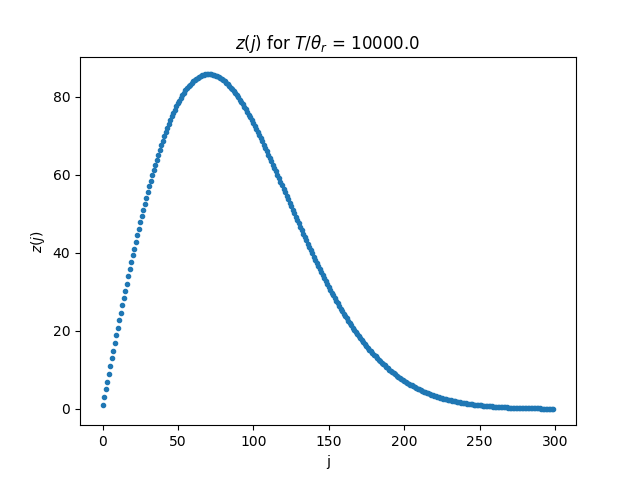
\includegraphics[scale=0.5]{e_stor.png}
\caption{A bar plot showing the terms of the partition function for $T/\theta_r >> 1$.}
\end{figure}\label{fig:large}

\begin{figure}[H]
\centering
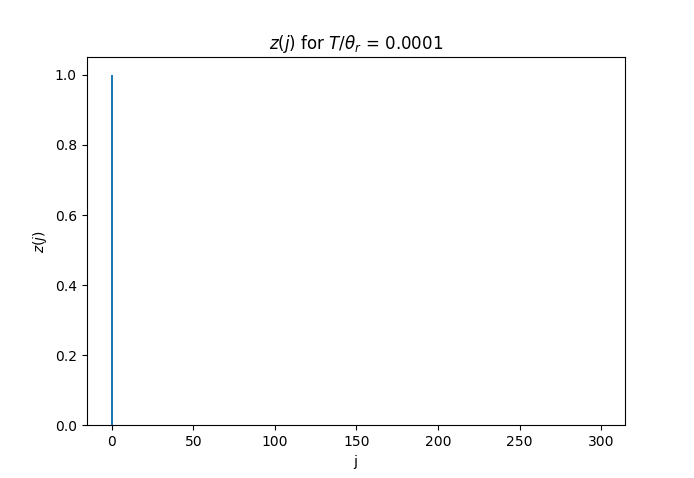
\includegraphics[scale=0.5]{e_liten.png}
\caption{A bar plot showing the terms of the partition function for $T/\theta_r << 1$.}
\end{figure}\label{fig:small}

We can see that for large values for $T/\theta_r$ terms for large values of $j$ contribute, but for small values of $T/\theta_r$  the only term that contributes is $z(0) = 1$ and the rest goes to zero.


\subsection{f)}
We can see in fig. \ref{fig:large} that when $T >> \theta_r$ that we can make a good approximation of the terms $z(j)$ as a continuous function, and therefore let the eq. \eqref{eq:partitionD} go towards an integration:

\begin{equation}
Z_r \approx \int_0^\infty (2j + 1) e^{-j(j+1)\theta_r/T} dj
\end{equation}\label{eq:large}

To solve this integral we use the change of variable

\begin{equation}
x = j(j+1) = j^2 + j, \qquad \frac{dx}{dj} = 2j + 1 \Rightarrow dj = \frac{dx}{2j+1}
\end{equation}

To the integral becomes

\begin{equation}
Z_r \approx \int_0^\infty e^{-x\theta_r/T} dx = -\frac{T}{\theta_r}e^{-x\theta_r/T} \bigg|_0^\infty = \frac{T}{\theta_r}
\end{equation}\label{eq:ZhightT}


So in the limit $T >> \theta_r$ $Z_r(T) = T/\theta_r$.


\subsection{g)}

For the limit $T << \theta_r$, we can see from fig. \ref{fig:small} that only the first term contribute. So we only need to write out the first few terms of eq. \eqref{eq:partitionD}:

\begin{equation}
Z_r \approx 1 + 3e^{-2\theta_r/T}
\end{equation}\label{eq:ZlowT}

The rest of the term goes very rapidly to zero, and is unnecessary to use.

\subsection{h)}
\subsubsection{High T}
For the high temperature approximation we can use eq. \eqref{eq:magic} to get

\begin{equation}
\langle E \rangle = -\pd{\ln Z}{\beta} = -\frac{1}{Z}\pd{}{\beta}Z = - \beta k \theta_r \pd{}{\beta} \frac{1}{\beta k \theta_r}
\end{equation}
\begin{equation}
= \beta k \theta_r \frac{1}{\beta^2 k \theta_r} = \frac{1}{\beta} = kT
\end{equation}\label{eq:highTE}

So for high temperature $\langle E \rangle= kT$

\subsubsection{Low T}
We again use eq. \eqref{eq:magic}:

\begin{equation}
\langle E \rangle = -\pd{}{\beta}\ln 1 +3e^{-2\theta_r k\beta}  = \theta_r k\frac{6e^{-2\theta_r k\beta}}{1 +3e^{-2\theta_r k\beta} } = \frac{6\theta_r k}{e^{2\theta_r/T} + 3}
\end{equation}\label{eq:lowTE}

So for low temperatures $\langle E \rangle = \frac{6\theta_r k}{e^{2\theta_r/T} + 3}$


\subsection{i)}

To find the heat capacity we use eq. \eqref{eq:heatCap}:

\subsubsection{High T}
For high temperatures we use eq. \eqref{eq:highTE} and find the heat capacity

\begin{equation}
C_v = \pd{}{T} kT = k
\end{equation}

So for high temperatures the hear capacity is simply $C_v = k$

\subsubsection{Low T}
For low temperatures we use eq. \eqref{eq:lowTE}. First we do a change of variable $\beta = 1/kT$

\begin{equation}
C_v = \pd{\beta}{T}\pd{}{\beta} \frac{6\theta_r k}{e^{2\theta_rk\beta} + 3} = \frac{-1}{kT^2}\frac{6\theta_r k e^{2\theta_rk\beta}\cdot 2\theta_r k }{\left(e^{2\theta_rk\beta} + 3\right)^2} = 
\frac{12\theta_r^2 k e^{2\theta_r/T}\cdot  }{T^2\left(e^{2\theta_r/T} + 3\right)^2}
\end{equation}

So for low temperatures the heat capacity is $C_v = \frac{12\theta_r^2 k e^{2\theta_r/T}\cdot  }{T^2\left(e^{2\theta_r/T} + 3\right)^2}$

\subsection{j)}
The function can be found at the end as \textbf{j.py}(\ref{sec:codeJ}).

\subsection{k)}
This also uses the code found in \textbf{j.py}(\ref{sec:codeJ}), and is the first plot:

\begin{figure}[H]
\centering
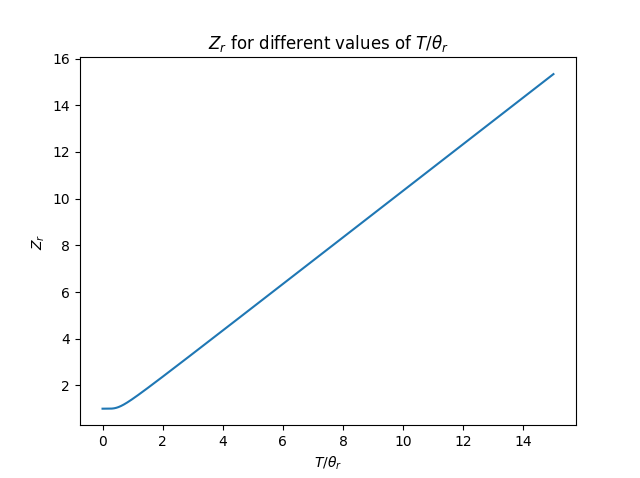
\includegraphics[scale=0.5]{k.png}
\caption{The partition function $Z_r$ for different values of $T/\theta_r$}
\end{figure}

We can see that near $T/\theta_r = 0$ $Z_r$ is constantly $\backsim 1$, but for larger values of $T/\theta_r$ $Z_r$ becomes a linear function. This is exactly what we found in \eqref{eq:ZlowT} and \eqref{eq:ZhightT}.

\subsection{l)}

The code for this is the second plot in \textbf{j.py}(\ref{sec:codeJ}), but is plotted with $T/\theta_r$ up to $200$.

\begin{figure}[H]
\centering
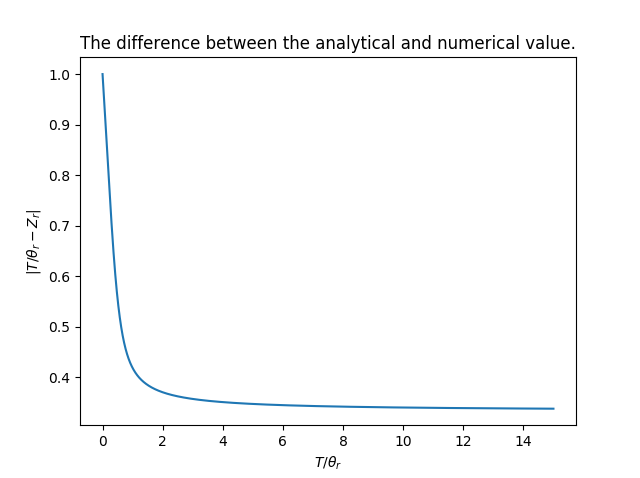
\includegraphics[scale=0.5]{diff_k.png}
\caption{Shows the difference between the analytical value for high temperature and the numerical value of the partition function.}
\end{figure}\label{fig:diff}

We can see from the above plot that the difference between the analytical value for high temperature and the numerical value for the partition function quickly decreases for higher values of $T/\theta_r$, but seems to flatten out around $1/3$. This is because we try to approximate a discrete function with a continuous one, which means that an integral will either over- or undershoot the real value. If we had drawn the continuous function on top of the bar plot in fig. \ref{fig:large} we would see that many bars had area outside over that function, meaning that in this case analytical value is about $1/3$ lower than the numerical value(This is printed out when running the code).


\subsection{m)}

To find the energy numerically we use that

\begin{equation}
\langle E\rangle = \frac{\sum_j E(j)e^{-\beta E(j)}}{Z} = \frac{\sum_j j(j+1)\theta_rk (2j + 1) e^{-j(j+1)\theta_r/T_i}}{\sum_j (2j + 1) e^{-j(j+1)\theta_r/T_i}} = E(T_i)
\end{equation}

Since the heat capacity \eqref{eq:heatCap} is defined with a differentiation, we have to use a numerical differentiation to find it.

To get most precision we use the symmetric difference quotient:

\begin{equation}
f'_i = \frac{f_{i+1} - f_{i-1}}{2h}
\end{equation}

And thus

\begin{equation}
C_v = \frac{1}{2h}(E(T_{i+1} )- E(T_{i-1})
\end{equation}	

\subsection{n)}
The code can be found at the end as \textbf{n.py}(\ref{sec:codeN})
\subsubsection{Energy}
\begin{figure}[H]
\centering
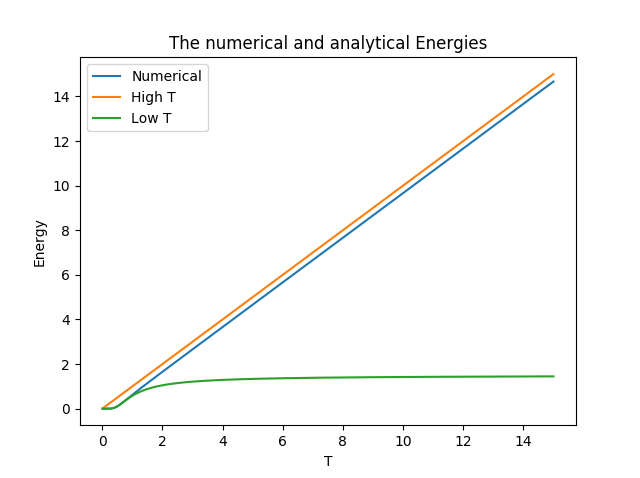
\includegraphics[scale=0.5]{n_E.png}
\caption{The numerical and analytic energies for different T}
\end{figure}	

As we can see, for low temperature the analytical and numerical solutions are in agreement, but for our high temperature solution the numerical solution is a constant higher than the analytic. This is stark contrast with the partition function where it was lower.


\subsubsection{Energy}
\begin{figure}[H]
\centering
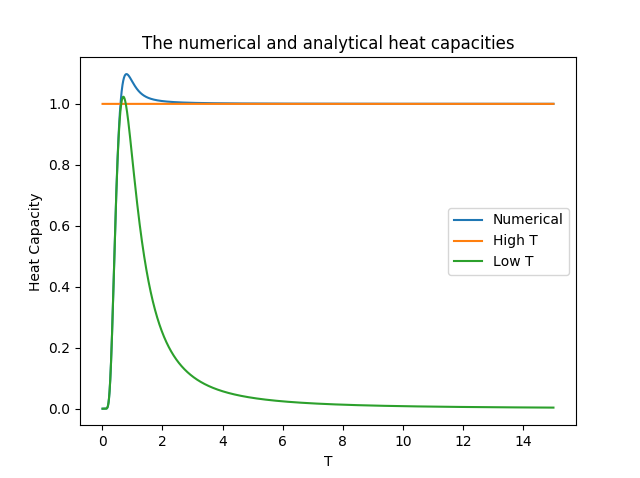
\includegraphics[scale=0.5]{n_cv.png}
\caption{The numerical and analytic heat capacities for different T}
\end{figure}

We can that the analytical and numerical solutions are good fits in their own domains. The constant difference for the high temperature is now gone, this is because for the energies the solutions were linear with a constant difference. Heat capacity is the derivative of the energies, meaning that this constant difference is differentiated away.

\section{Codes}
\subsection{c.py}\label{sec:codeC}
\lstinputlisting{c.py}

\subsection{e.py}\label{sec:codeE}
\lstinputlisting{e.py}

\subsection{j.py}\label{sec:codeJ}
\lstinputlisting{j.py}

\subsection{n.py}\label{sec:codeN}
\lstinputlisting{n.py}
\end{document}

